\section{Motivation}
\label{sec:motivation}


\subsection{Limits of Source-Only LLM Reasoning}
\label{subsec:llm-limitations}

The remaining question is empirical: once the HLS objective and target are made explicit, how much of the hardware-relevant structure can a strong decoder-only LLM recover from source tokens alone?

We study Pathfinder and Viterbi as a controlled increase in source and directive complexity. Pathfinder has McCabe cyclomatic complexity
5~\cite{mccabe1976complexity}, four actions, ten directive fields and $1.76\times10^{13}$ source-legal assignments; Viterbi has complexity 11, eight actions, seventeen fields, and $1.03\times10^{18}$ assignments. We use cyclomatic complexity only
as a source-level descriptor, not as a proxy for HLS difficulty.

We evaluate GPT-5.6 Sol, Claude Opus 5, and Gemini 3.1 Pro Preview under three one-pass prompting regimes. \emph{Free-form} prompting provides the kernel, local header context, device, clock, resource limits, and latency objective but leaves pragma placement and values to the model. \emph{Action+domain} additionally exposes the exact source-derived loop/array action sites and finite RHS proposal domains. Finally, \emph{Action+domain+RAG} augments the same structured prompt with the five most relevant HLS guidance entries from a frozen, HLSPilot-inspired corpus. The RAG corpus contains general pipeline, unrolling, partitioning, memory bandwidth, and dependence guidance, but no GN$\Omega$SIS QoR values, Pareto configurations, \framework outputs, or synthesis feedback. Thus the three regimes progressively remove placement, domain, and textual-knowledge confounds while never exposing compiler-graph structure.

\begin{figure*}[t]
    \centering
    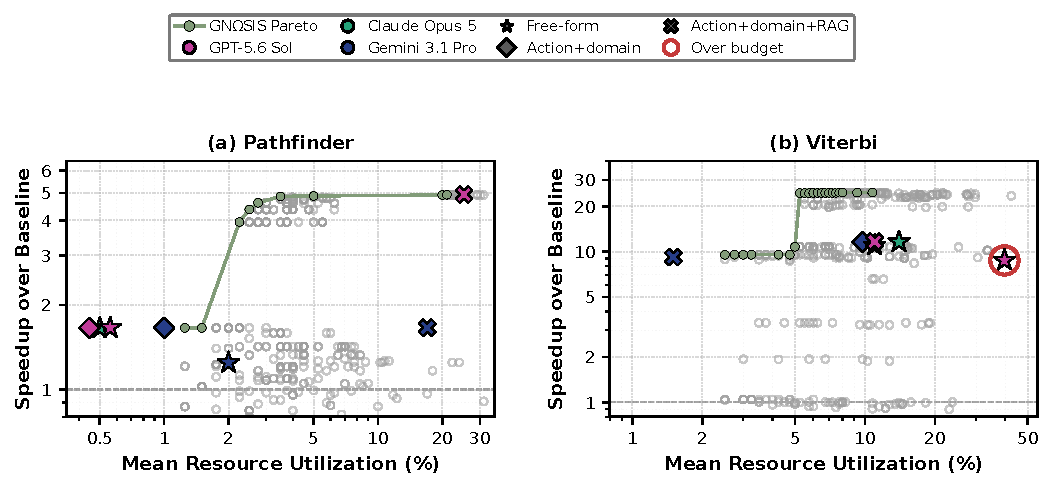
\includegraphics[
        width=0.82\textwidth
    ]{figures/03__Motivation/motivation_pathfinder_viterbi_FINAL.pdf}
    \caption{\textbf{General-purpose LLMs under progressively stronger HLS prompting on Pathfinder and Viterbi.}
    Synthesized designs are compared with the measured GN$\Omega$SIS Pareto frontier~\cite{ferikoglou2026gnomegasis}; red circles denote component-wise resource infeasibility.}
    \label{fig:llm-decoder-limitation}
\end{figure*}

The contrast is not simply a syntax effect. On Pathfinder, the best hosted model reaches $4.94\times$ speedup and lies close to the measured latency-efficient frontier. On Viterbi, the best synthesized hosted-model configuration reaches $11.64\times$, while the measured frontier extends to roughly twice that speedup at comparable or lower resource utilization. 
Moreover, five of the twelve action-structured outputs violate the required assignment schema despite receiving the legal action sites and value domains. Among the thirteen configurations that proceed to synthesis, twelve are component-wise feasible; the remaining Viterbi free-form configuration reaches 103\% LUT utilization. Providing legal action sites therefore removes one source of ambiguity, but does not make prompt-only generation either structurally grounded or reliably constraint aware.


\subsection{Pitfalls of Structure-Agnostic Adaptation}

The three prompting regimes isolate what textual assistance can and cannot supply. Exposing action sites eliminates the need to discover pragma placement; exposing domains provides legal candidate values; and RAG adds explicit HLS knowledge about pipelining, unrolling, partitioning, dependences, and memory bandwidth. These interventions can improve individual decisions---most clearly for GPT-5.6 Sol on Pathfinder---but the information remains an unstructured token sequence. The model must still determine which dependence constrains which loop, which memory object supplies an unrolled computation, and which other directive decisions share that structure.

The missing signal is therefore more specific than generic ''long-range attention.'' HLS decisions need an explicit correspondence between a source action and the compiler relations that determine its hardware effect. This motivates \framework's Stage~2 design: preserve the semantic and target-aware policy learned from source code, but expose each directive decision to compiler-derived memory aligned to the same action identity. The following sections describe how this alignment is constructed and test whether it---rather than additional prompting, output constraints, or model capacity---accounts for the resulting QoR.